
\section{Goals for today}
By the end of this lecture, you should be able:
\begin{enumerate}
\item Apply signals and systems properties to reason about real-world systems.
\item To understand how to compute the output of a linear-time invariant system given any general input signal that is applied to the system. 
\end{enumerate}

\section{Review: Signals and Systems}
Recall that signals are mathematical functions that represent physical quantities, or information. Usually, we may think of signals as functions of time, but they can also be functions of space or other variables. A simple rule of thumb to remember is that signals are mathematical functions (that you can also visualize, if they are 1D or 2D).

On the other hand, you can easily distinguish systems from signals because systems are ``processors'' of signals. Every quantity/information/measurement is a signal, and systems can process a signal to produce an output signal. The signal that gets processed by the system is the input signal and the processed signal is the output signal. Due to this, a common abstraction of a system is a ``black box'' that takes in an input signal and produces an output signal. Formally, we write a system as an operator (or a mapping) that takes in a signal and produces another signal:
\[
    H: x(t) \mapsto y(t) 
\]
where $x(t)$ is the input signal, $y(t)$ is the output signal, and $H$ is the system. Note that the above does not imply that $x(t) = y(t)$, and in fact, if the system is doing something meaningful, the output signal will be different from the input signal. System examples:
\subsection{Example: A matrix as a system}
Given an input vector $x \in \mathbb{R}^n$, a matrix $A \in \mathbb{R}^{m \times n}$ can be thought of as a system that produces an output vector $y \in \mathbb{R}^m$ as follows:
\[
    y = Ax
\]
where $A$ is the system that performs the matrix multiplication operation. The block diagram of the system can be represented as:
\begin{figure}[h]
\centering
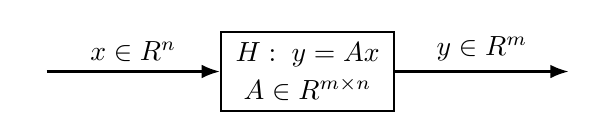
\begin{tikzpicture}[node distance=2.2cm]
  \node (in) {};
  \node[block, right=of in] (A) {$H:\; y=Ax$ \\[2pt] $A\in\mathbb{R}^{m\times n}$};
  \node[right=of A] (out) {};
  \draw[conn] (in) -- node[above] {$x\in\mathbb{R}^n$} (A);
  \draw[conn] (A) -- node[above] {$y\in\mathbb{R}^m$} (out);
\end{tikzpicture}
\caption{A system as a linear map implemented by matrix multiplication.}
\end{figure}

\subsection{Example: An amplifier as a system}
An amplifier is a system that takes in an input signal $x(t)$ and produces an output signal $y(t)$ by amplifying the input signal by a constant factor $\alpha \in \mathbb{R}$. The system can be represented as:
\[
    H: x(t) \mapsto y(t) = \alpha x(t)
\]
where $H$ is the system that amplifies the input signal by the factor $\alpha$. We can draw a block diagram of the system as follows:
\begin{figure}[h]
\centering
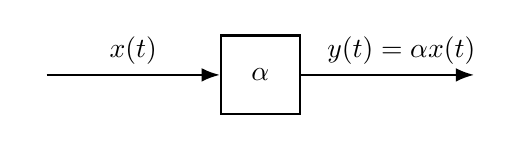
\begin{tikzpicture}[node distance=2.2cm]
  \node (xin) {};
  \node[gain, right=of xin] (G) {$\alpha$};
  \node[right=of G] (yout) {};
  \draw[conn] (xin) -- node[above] {$x(t)$} (G);
  \draw[conn] (G) -- node[above] {\quad $y(t)=\alpha x(t)$} (yout);
\end{tikzpicture}
\caption{Amplifier system: multiply the input by a real gain \(\alpha\).}
\end{figure}
\subsection{Example: A differential equation as a system}
A system can also be represented by a differential equation that relates the input signal $x(t)$ and the output signal $y(t)$. For example, consider the following first-order linear differential equation:
\[
    \frac{dy(t)}{dt} + ay(t) = bx(t)
\]
where $a$ and $b$ are constants. This equation describes a system that takes in the input signal $x(t)$ and produces the output signal $y(t)$ by solving the differential equation.
In this case, the block diagram of the system can be represented as:
% put once in preamble
\usetikzlibrary{arrows.meta,positioning,calc}
\tikzset{
  >={Latex[length=2mm]},
  block/.style={draw, thick, rectangle, minimum height=10mm, minimum width=22mm, align=center},
  gain/.style={block, minimum width=10mm},
  sum/.style={draw, thick, circle, inner sep=0pt, minimum size=6mm},
  conn/.style={-Latex, thick},
}

% figure
\begin{figure}[h]
\centering
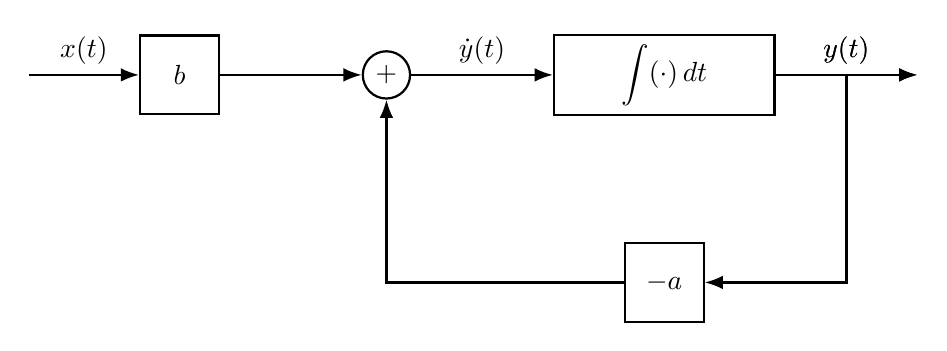
\begin{tikzpicture}[node distance=14mm]
  % nodes
  \node[coordinate] (xin) {};
  \node[gain, right=of xin] (Gb) {$b$};
  \node[sum, right=18mm of Gb] (sum) {$+$};
  \node[block, right=18mm of sum, minimum width=28mm] (Int) {$\displaystyle \int(\cdot)\,dt$};
  \node[coordinate, right=18mm of Int] (yout) {};
  \node[gain, below=16mm of Int] (Ga) {$-a$};

  % connections
  \draw[conn] (xin) -- node[above] {$x(t)$} (Gb.west);
  \draw[conn] (Gb.east) -- (sum.west);
  \draw[conn] (sum.east) -- node[above] {$\dot y(t)$} (Int.west);
  \draw[conn] (Int.east) -- node[above] {$y(t)$} (yout);

  % feedback path (tap from integrator output)
  % % get feedback path from middle of the yout arrow
\draw[conn] (Int.east) -- node[above] {$y(t)$} coordinate[pos=0.5] (ytap) (yout);
\draw[conn] (ytap) |- (Ga.east);
  \draw[conn] (Ga.west) -| (sum.south);
  % optional plus labels at summer inputs (the - sign is in the feedback gain)
  % \node at ($(sum)+(-0.35,0.28)$) {\scriptsize $+$};
  % \node at ($(sum)+(-0.35,-0.30)$) {\scriptsize $+$};
\end{tikzpicture}
\caption{Realization of \(\dot y(t)+a\,y(t)=b\,x(t)\).}
\end{figure}

\subsection{Example: A frequency modulation system}
A frequency modulation (FM) system is a system that takes in an input signal $x(t)$ and produces an output signal $y(t)$ by modulating the frequency of a carrier signal. 

\begin{popquiz}
For a purely sinusoidal audio signal $x(t) = A\cos(\omega_0 t)$, define a frequency modulator system that produces an output signal $y(t)$ that has a different frequency than the input signal. What are various ways in which you can achieve this? Can you think of a general approach to create such a system by leveraging the properties of the complex exponential signal (see previous chapter of the notes)?
\popqsplit
If you define the system as a multiplication of the input signal with $\Re\{A e^{j\omega_0 t}\}$, you will see that the output signal has a frequency that is shifted by $\omega_0$ from the input signal. 
\end{popquiz}
Consider a specific example where $x(t) = e^{j 2 \pi (10 t)}$ and we send this input through a modulator system that multiplies $e^{j 2 \pi (32 t)}$ to the input signal. The output can be obtained by computing the shift in frequency (exponents get added on multiplication). The output signal $y(t)$ for both the real and imaginary parts of the complex exponential modulator system is shown in Figure~\ref{fig:fm_sine}. 
\begin{figure}[ht]
    \centering
    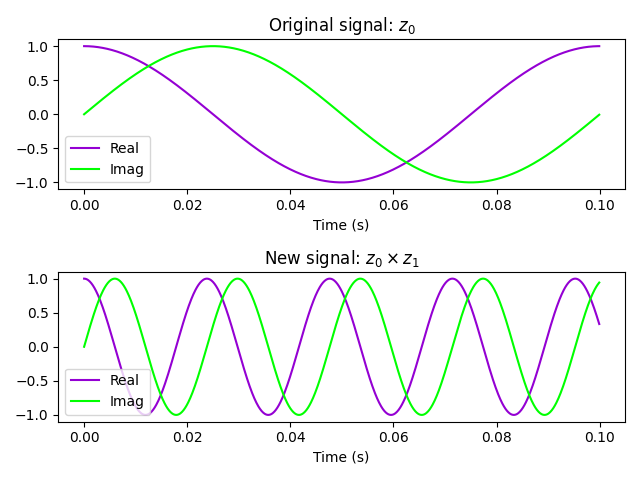
\includegraphics[width=\textwidth]{figs/fm_sine.png} 
    \caption{Frequency modulation of a sinusoidal signal using multiplication with a complex exponential.}
    \label{fig:fm_sine}
\end{figure}

An audio signal can be thought of as a combination of many sinusoidal signals with different frequencies. So, we can leverage the properties of the general complex exponential signal to define the input audio signal $x(t)$ as a sum of complex exponentials:
\[
    x(t) = \sum_{k} \Re\left(A_k e^{j\omega_k t}\right)
\]
where $A_k$ and $\omega_k$ are the amplitude and frequency of the $k$-th sinusoidal component of the audio signal. Note that for simplicity, we are just considering the cosine component. To keep it general, we can continue to work with complex numbers as it allows us to take into account both sine and cosine components (orthogonally phase shifted by $\pi/2$, which is important in representing a general signal). If we define our system as a multiplication of the input signal with $\Re\{A e^{j\omega_0 t}\}$, we will see that the output signal has a frequency that is shifted by $\omega_0$ from the input signal. The system can be represented as:
\[
    H: x(t) \mapsto y(t) = x(t) \cdot \Re\{A e^{j\omega_0 t}\}
\]
where $H$ is the system that modulates the frequency of the input signal by multiplying it with a carrier signal $\Re\{A e^{j\omega_0 t}\}$. In this case, the output $y(t)$ can be written as a sum of sinusoidal signals with frequencies shifted by $\omega_0$:
\[
    y(t) = \sum_{k} \Re\left(A_k e^{j(\omega_k + \omega_0) t}\right)
\]
For a real audio signal that you can find on course Github: \href{https://github.com/ee-ucmerced/ee102-signals-systems/blob/main/lecture\_notes/week3\_special\_signals/guitar\_clean.wav}{guitar\_clean.wav}, we can create the simple frequency modulator using the multiplication of a complex exponential. The input and the output signals are shown in Figure~\ref{fig:fm_guitar}. You can interactively visualize and interpret the frequency of the output signal by running the virtual manipulator on frequency modulator using complex exponentials: \href{https://github.com/ee-ucmerced/ee102-signals-systems/blob/main/lecture\_notes/week3\_special\_signals/VM\_modulation.py}{VM\_modulation.py}.
\begin{figure}[ht]
    \centering
    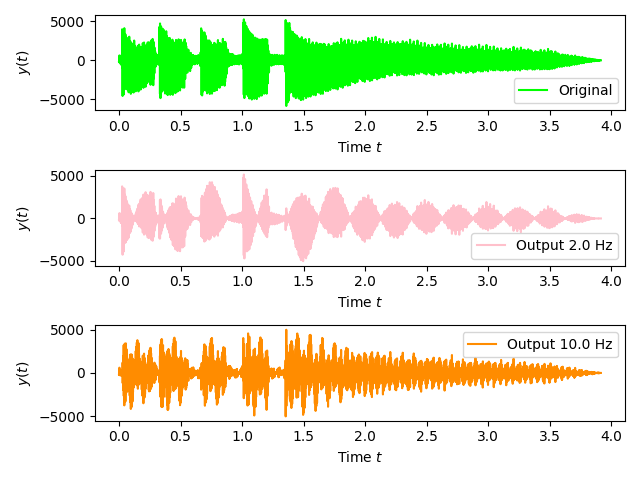
\includegraphics[width=\textwidth]{figs/fm_guitar.png} 
    \caption{Frequency modulation of a guitar audio signal using multiplication with a complex exponential.}
    \label{fig:fm_guitar}
\end{figure}
\begin{popquiz}
  By using the virtual manipulator \href{https://github.com/ee-ucmerced/ee102-signals-systems/blob/main/lecture\_notes/week3\_special\_signals/VM\_modulation.py}{VM\_modulation.py}, test three different frequencies of the modulator system: 0.5 Hz, 5 Hz, and 20 Hz. Reflect on the expected sound for each modulation before listening to the output \texttt{guitar\_modulated.wav}. Which one of the output signals is closest to the original audio signal? How would you describe the frequency modulation effect on audio?
  \popqsplit
  The 0.5 Hz modulation is closest to the original audio signal. The frequency modulation effect on audio can be described as a shift in the frequency spectrum of the original signal, resulting in a change in the perceived pitch and timbre of the sound, which ends up sounding like a reverberation.
\end{popquiz}
\begin{popquiz}
  Can you define a noise cancellation system that takes in a noisy signal and produces an output signal that cancels the noise? Assume that the noise is a sinusoidal signal with a known frequency and amplitude. 
  \popqsplit
  See Problem Set \#3.
\end{popquiz}

\section{LTI Output}
\subsection{Example: LTI system response}
By using linearity and time-invariance, we can analyze the response of an LTI system to inputs and initial conditions. Consider the system with three different inputs: $x_1(t)$, $x_2(t)$, and $x_3(t)$. Define the output of the system for each of the signals as $y_1(t)$, $y_2(t)$, and $y_3(t)$ respectively. Let us assume that the system is also affected by its initial conditions $q_1(0)$ and $q_2(0)$. 

We denote $y_i^{\mathrm{ZS}}(t)$ as the zero-state output due to $x_i(t)$ with all initial conditions set to zero. Further, we denote $y_{q_1}(t)$ and $y_{q_2}(t)$ as the zero-input outputs produced by initial conditions in those two modes (with external inputs, $x_i$, set to zero).

Then, for any scalars $\alpha_1,\dots,\alpha_5$,
\[
x(t)=\alpha_1 x_1(t)+\alpha_2 x_2(t)+\alpha_3 x_3(t),\quad
q(0)=\alpha_4\,q_1(0)+\alpha_5\,q_2(0)
\]
\[
~\Longrightarrow~
y(t)=\alpha_1 y_1^{\mathrm{ZS}}(t)+\alpha_2 y_2^{\mathrm{ZS}}(t)+\alpha_3 y_3^{\mathrm{ZS}}(t)
      +\alpha_4 y_{q_1}(t)+\alpha_5 y_{q_2}(t).
\]
Note that it is essential that $y_i^{\mathrm{ZS}}$ are computed with zero initial conditions otherwise the initial contributions would be double-counted. Likewise, $y_{q_1},y_{q_2}$ are computed with zero external input.

Further, if one of the inputs is shifted in time, say $x_3(t-t_0)$, then by the time-invariance property of the system, the output is also shifted by the same amount:
\[
x(t)=\alpha_1 x_1(t)+\alpha_2 x_2(t)+\alpha_3 x_3(t-t_0),\quad
q(0)=\alpha_4\,q_1(0)+\alpha_5\,q_2(0)
\]
\[
~\Longrightarrow~
y(t)=\alpha_1 y_1^{\mathrm{ZS}}(t)+\alpha_2 y_2^{\mathrm{ZS}}(t)+\alpha_3 y_3^{\mathrm{ZS}}(t-t_0)
      +\alpha_4 y_{q_1}(t)+\alpha_5 y_{q_2}(t).
\]
\subsection{Example: LTI system properties to compute system response}

Consider a continuous-time LTI system with input $x(t)$ and output $y(t)$. We have the following information about the system:
\[
\begin{aligned}
x_1(t)&=\cos(t) 
&&\longrightarrow&&
y_1(t)=\tfrac{1}{10}\cos(t)-\tfrac{3}{10}\sin(t),\\[2pt]
x_2(t)&=\cos(2t) 
&&\longrightarrow&&
y_2(t)=\tfrac{1}{5}\cos(2t)+\tfrac{3}{10}\sin(2t),\\[2pt]
x_3(t)&=\delta(t)
&&\longrightarrow&&
y_3(t)=\delta(t),\\[2pt]
\end{aligned}
\]

Then, for a new input
\[
x_{\text{new}}(t)=\cos(2t)-10\sin(t+10),
\]
our goal is to find $y_{\text{new}}(t)$ using only linearity and time invariance properties of the system. 

Let us start by noting that since $\sin(t)=\cos\!\big(t-\tfrac{\pi}{2}\big)$, we can use time-invariance of the system to write the output for $\sin(t)$ (say $y_4(t)$) as
\[
y_4(t)=y_1\!\Big(t-\tfrac{\pi}{2}\Big)
=\tfrac{1}{10}\sin(t)+\tfrac{3}{10}\cos(t).
\]
Then, the output to $\sin(t+10)$ is (say $y_5(t)$), again due to time-invariance is obtained by shifting $y_4(t)$ by $10$:
\[
\begin{aligned}
y_5(t)
&=\tfrac{1}{10}\sin(t+10)+\tfrac{3}{10}\cos(t+10)
\end{aligned}
\]
Putting it all together using the linearity of the system, we get the desired output $y_{\text{new}}(t)$:
\[\,y_{\text{new}}(t)
=\tfrac{1}{5}\cos(2t)+\tfrac{3}{10}\sin(2t)\;-\;\sin(t+10)\;-\;3\cos(t+10)\,.
\]

Finally, if the system has an initial condition at $t=0$, superpose the corresponding measured responses:
\[
\,y_{\text{new,IC}}(t)=y_{\text{new}}(t)\;+\;a\,\delta(t)\,,
\]
with $a \in\mathbb{R}$ set by the magnitude of the initial condition.

\textbf{\color{red}BUT...}
\begin{popquiz}
Show that the problem above is internally inconsistent. That is, it is not possible for an LTI system to have the impulse response $y_3(t)=\delta(t)$ and the other responses $y_1(t)$ and $y_2(t)$ as given.

\popqsplit
A simple proof by counterexample is enough. For an LTI system, the response to \(\delta(t)\) is the impulse response. Thus,
$
h(t)=\delta(t).
$
The output for any input \(x(t)\) is therefore
$
y(t)=x(t)*h(t)=x(t)*\delta(t)=x(t).
$

Hence, \(x_1(t)=\cos(t)\) must produce \(y_1(t)=\cos(t)\), which contradicts the given
$
y_1(t)=\frac{1}{10}\cos(t)-\frac{3}{10}\sin(t).
$
Therefore, the given input-output pairs cannot all correspond to the same LTI system.
\end{popquiz}
\section{Representing signals using impulses}
We have discussed the three fundamental signals: the unit step, the unit impulse, and the complex exponential. What's common about all three of these functions? Why are these three signals so special? The answer is that these three signals can be used to represent any arbitrary signal (well, almost any!) --- especially the signals that we come across in engineering practice. In the previous lectures, we have discussed how to write general signals only by using unit steps and complex exponentials. We have also briefly discussed how the definition of the unit impulse (in the sense of distributions), is in fact, a definition that says that each signal is made up of its samples at each time point and the impulse is the function that does the sampling. Let's try to break this down further with some examples. 

\subsection{Discrete-time step using impulse}
To help you build intuition for this concept, consider a signal in discrete-time. For example, the unit step signal $u[n]$ is defined as
\[
u[n] = \begin{cases}
1, & n \geq 0 \\
0, & n < 0
\end{cases}
\]
which can be visualized as a train of unit impulses as shown in Figure \ref{fig:d-t-unit-step}. It is clear that it is a signal that is made up of many impulses (see pop quiz below).

\begin{popquiz}
In discrete-time, write the unit step signal $u[n]$ as a sum of scaled and shifted unit impulses $\delta[n]$. 
\popqsplit
Notice that for any given value of $n$, the unit step $u[n]$ is equal to 1 if $n \geq 0$ and 0 otherwise. This means that the unit step can be viewed as a sum of all the unit impulses $\delta[k]$ for $k$ from $-\infty$ to $n$. So, we can write
\[
u[n] = \sum_{k=-\infty}^{n} \delta[k]
\]
for all $n \in \mathbb{Z}$. To represent the signal in terms of the general impulse $\delta[n]$, we can write:
\[
u[n] = \sum_{k=0}^{\infty} \delta[n-k].
\]
You can see that for any given $n$, the sum will only include the impulses from $k=0$ to $k=n$, which corresponds to the definition of the unit step. 
\end{popquiz}
\begin{figure}[h]
\centering
\begin{tikzpicture}[scale=1.0]
    % Draw axes
    \draw[->] (-5,0) -- (5,0) node[right] {$n$};
    \draw[->] (0,-1) -- (0,3) node[above] {$u[n]$};

    % Draw unit step
    \foreach \x in {0,1,2,3,4} {
        \draw[thick] (\x,0) -- (\x,2);
        \filldraw[black] (\x,2) circle (2pt);
    }
    \draw[thick] (-5,0) -- (0,0);
    \filldraw[black] (0,2) circle (2pt);

    % Add labels
    \node at (1,-0.5) {1};
    \node at (2,-0.5) {2};
    \node at (3,-0.5) {3};
    \node at (4,-0.5) {4};
    \node at (-1,-0.5) {-1};
    \node at (-2,-0.5) {-2};
    \node at (-3,-0.5) {-3};
    \node at (-4,-0.5) {-4};
    \node at (0.5,2.5) {};
\end{tikzpicture}

\caption{Unit step signal $u[n]$ visualized as a train of unit impulses.}
\label{fig:d-t-unit-step}
\end{figure} 


We see that the unit step can be viewed as many impulses (one impulse at each time point). This is also true for every other signal --- the simplest way to break down a signal is to view it as a sample at each time point. The unit impulse helps us pick out the samples at each time point so that we can write the logic above formally. A visualization of this idea is shown in Figure~\ref{fig:dt-impulse-sum}. 

\begin{figure}[h]
\centering

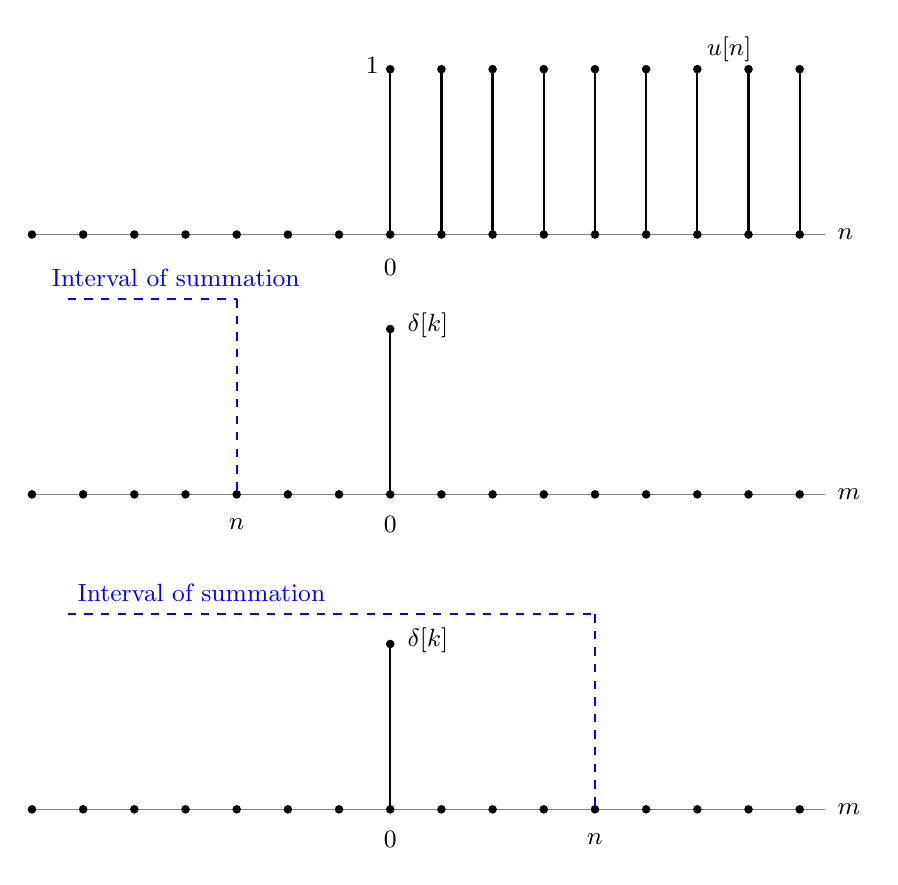
\begin{tikzpicture}[>=stealth, x=0.65cm, y=2.1cm]
  \tikzset{
    dot/.style={circle, fill=black, inner sep=1.1pt},
    stem/.style={thick},
    dashint/.style={blue, dashed, thick},
    axisline/.style={gray},
    txt/.style={font=\small}
  }

  \def\xmin{-7}  \def\xmax{8}
  \def\nmarkL{-3} % panel 2: n is to the LEFT of 0
  \def\nmarkR{4}  % panel 3: n is to the RIGHT of 0

  \begin{scope}[yshift=1.8cm]
    \draw[axisline] (\xmin,0) -- (\xmax+0.5,0);
    \foreach \k in {\xmin,...,\xmax} \node[dot] at (\k,0) {};
    % unit step u[n]
    \foreach \k in {0,...,\xmax} {
      \draw[stem] (\k,0) -- (\k,1);
      \node[dot] at (\k,1) {};
    }
    % labels
    \node[txt,anchor=west] at (\xmax+0.55,0) {$n$};
    \node[txt] at (-0.35,1.02) {$1$};
    \node[txt] at (0,-0.2) {$0$};
    \node[txt,anchor=west] at (6.0,1.12) {$u[n]$};
  \end{scope}


  \begin{scope}[yshift=-1.5cm]
    \draw[axisline] (\xmin,0) -- (\xmax+0.5,0);
    \foreach \k in {\xmin,...,\xmax} \node[dot] at (\k,0) {};
    % impulse δ[m]
    \draw[stem] (0,0) -- (0,1);
    \node[dot] at (0,1) {};
    \node[txt,anchor=west] at (0.15,1.02) {$\delta[k]$};
    \node[txt,anchor=west] at (\xmax+0.55,0) {$m$};
    % axis tick labels: n (left of 0) and 0
    \node[txt] at (\nmarkL,-0.18) {$n$};
    \node[txt] at (0,-0.18) {$0$};
    % blue dashed interval: from far left up to n (left of 0)
    \draw[dashint] (\xmin+0.7,1.18) -- (\nmarkL,1.18);
    \draw[dashint] (\nmarkL,1.18) -- (\nmarkL,0);
    \node[txt,anchor=west,blue] at (\xmin+0.2,1.31) {Interval of summation};
  \end{scope}
  \begin{scope}[yshift=-5.5cm]
    \draw[axisline] (\xmin,0) -- (\xmax+0.5,0);
    \foreach \k in {\xmin,...,\xmax} \node[dot] at (\k,0) {};
    % impulse δ[m]
    \draw[stem] (0,0) -- (0,1);
    \node[dot] at (0,1) {};
    \node[txt,anchor=west] at (0.15,1.02) {$\delta[k]$};
    \node[txt,anchor=west] at (\xmax+0.55,0) {$m$};
    % axis tick labels: 0 and n (right of 0)
    \node[txt] at (0,-0.18) {$0$};
    \node[txt] at (\nmarkR,-0.18) {$n$};
    % blue dashed interval: from far left up to n (right of 0)
    \draw[dashint] (\xmin+0.7,1.18) -- (\nmarkR,1.18);
    \draw[dashint] (\nmarkR,1.18) -- (\nmarkR,0);
    \node[txt,anchor=west,blue] at (\xmin+0.7,1.31) {Interval of summation};
  \end{scope}
\end{tikzpicture}

\caption{Visualization of the running sum representation of the unit step signal $u[n]$ as a sum of shifted impulses.}
\label{fig:dt-impulse-sum}
\end{figure}

\subsection{Impulse as a sampler in continuous-time}
Recall the sampling property of the impulse in continuous-time:
\[
\int_{-\infty}^{\infty} x(t) \delta(t - t_0) dt = x(t_0).
\]
This property tells us that the impulse function $\delta(t - t_0)$ acts as a sampler that picks out the value of the signal $x(t)$ at the specific time $t = t_0$. This means that we can represent any continuous-time signal $x(t)$ as an integral of scaled and shifted impulses. 
\subsection{Example: Representing a sinusoidal signal using impulses}
Let's work through this with a specific example of a sinusoidal signal: $x(t) = \sin(t)$. We can write $\sin(0)$ as
\[
\sin(0) = \int_{-\infty}^{\infty} \sin(\tau) \delta(\tau - 0) d\tau.
\]
Similarly, we can write $\sin(t_1)$ for any arbitrary time $t_1$ as
\[
\sin(t_1) = \int_{-\infty}^{\infty} \sin(\tau) \delta(\tau - t_1) d\tau.
\]
This means that we can represent the entire signal $\sin(t)$ as an integral of scaled and shifted impulses:
\[
\sin(t) = \int_{-\infty}^{\infty} \sin(\tau) \delta(\tau - t) d\tau.
\]
Now, this might seem trivial or even circular! But the key insight here is that we are expressing the signal as a continuous superposition of impulses, each weighted by the value of the signal at that point in time. 

\subsection{General representation of signals using impulses}
In general, any continuous-time signal $x(t)$ can be represented using impulses. Let's visualize an arbitrary signal $x(t)$ and see how it can be decomposed into impulses at each time point (see Figure~\ref{fig:ct-impulse-samplers}).
\begin{figure}[h]
\centering
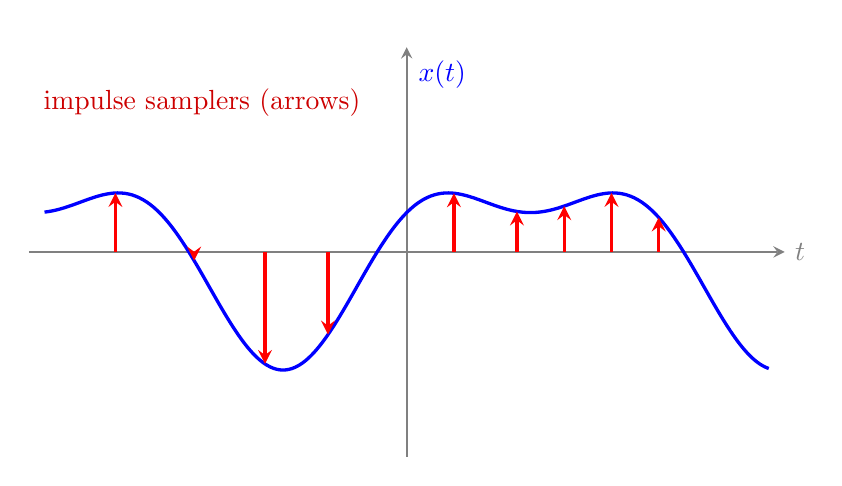
\begin{tikzpicture}[x=1cm,y=1cm,>=stealth]
  % --- axes ---
  \draw[->,gray,thick] (-4.8,0) -- (4.8,0) node[right] {$t$};
  \draw[->,gray,thick] (0,-2.6) -- (0,2.6) node[above] {};

  % --- signal x(t) ---
  \draw[very thick,blue,domain=-4.6:4.6,samples=200,smooth,variable=\t]
        plot ({\t},{sin(\t r) + 0.5*cos(2*\t r)});
  \node[blue] at (0.45,2.25) {$x(t)$};
  \node[red!80!black] at (-2.6,1.9) {impulse samplers (arrows)};

  % --- sampling instants ---
  \def\samples{-3.7,-2.7,-1.8,-1.0,0.6,1.4,2.0,2.6,3.2}

  % --- arrows that start on the x-axis and point to the curve ---
  \foreach \tt in \samples{
    \pgfmathsetmacro{\yy}{sin(\tt r) + 0.5*cos(2*\tt r)}
    % arrow from (t,0) to (t, y(t)), head at the curve
    \draw[red,very thick,-stealth] (\tt,0) -- (\tt,\yy);
  }
\end{tikzpicture}
\caption{Impulse samplers drawn as arrows from the time axis to the signal $x(t)$ (arrowheads at the curve).}
\label{fig:ct-impulse-samplers}
\end{figure}


At each point, the impulse signal can be written by shifting the impulse to that point and scaling it by the value of the signal at that point. Therefore, we start with $\delta(t)$ as the impulse at $t=0$. To get the impulse at an arbitrary time $t=\tau$, we shift the impulse to that point, which gives us $\delta(t - \tau)$. To scale this impulse by the value of the signal at that point, we multiply it by $x(\tau)$, resulting in $x(\tau) \delta(t - \tau)$. So, we have
\[
x(t) = \int_{-\infty}^{\infty} x(\tau) \delta(t - \tau) d\tau.
\]
\section{General output of an LTI system using impulse response}
We finally get to the main goal of this lecture. Our goal is to compute the output of systems given any arbitrary input signal. This is very important because in practice, we often encounter signals that are not as simple as the unit step or the complex exponential. We need a systematic way to compute the output of a system for any input signal. Think about the following examples, where we might want to compute the output of a system:
\begin{itemize}
    \item An audio signal (your recorded voice singing a song, for example) that needs to be filtered to remove noise. How would you represent your filtered signal mathematically (to be able to analyze and report back its properties to your music producer!)?
    \item For an integrated circuit, you might want to compute the output voltage of a circuit given an arbitrary input voltage signal (in real-world, the voltage signal is never a perfect sinusoid!).
    \item In communications, you might want to compute the output of a communication channel given an arbitrary input signal (for example, a modulated signal carrying information).
\end{itemize}
To achieve all of the above, we start by describing the impulse response of the system.

\subsection{Impulse response of an LTI system}
We define the impulse response of a system as the output of the system when the input is an impulse signal. In continuous-time, if the system input is $\delta(t)$, then we call the output of this system, the impulse response and denote it as $h(t)$ (see Figure~\ref{fig:impulse-response}).
\begin{figure}[h]
\centering
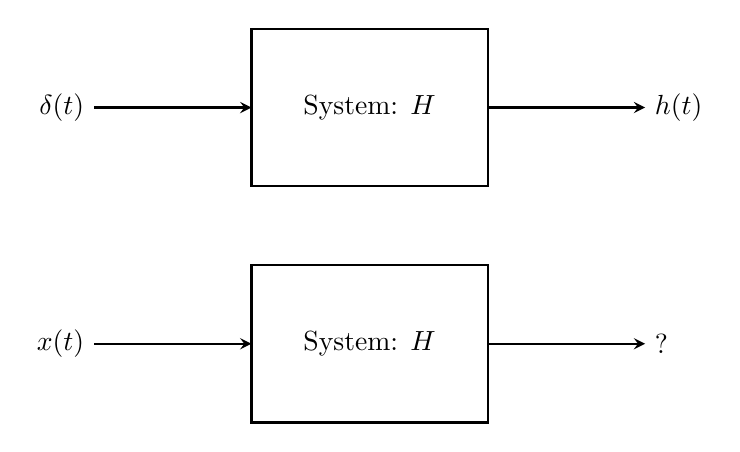
\begin{tikzpicture}[>=stealth, x=1cm, y=1
cm]
  % Draw the system box
  \draw[thick] (0,0) rectangle (3,2);
  \node at (1.5,1) {System: $H$};

  % Input arrow and label
  \draw[->, thick] (-2,1) -- (0,1);
  \node[anchor=east] at (-2,1) {$\delta(t)$};

  % Output arrow and label
  \draw[->, thick] (3,1) -- (5,1);
  \node[anchor=west] at (5,1) {$h(t)$};

  % add another box with x(t) input and ? output
    \draw[thick] (0,-3) rectangle (3,-1);
    \node at (1.5,-2) {System: $H$};
    % Input arrow and label
    \draw[->, thick] (-2,-2) -- (0,-2);
    \node[anchor=east] at (-2,-2) {$x(t)$};
    % Output arrow and label
    \draw[->, thick] (3,-2) -- (5,-2);
    \node[anchor=west] at (5,-2) {$?$};

    % Labels
    % \node at (1.5,2.3) {Impulse Response};
\end{tikzpicture}
\caption{Impulse response of a system: output $h(t)$ when input is $\delta(t)$. What is the output for a general input $x(t)$?}
\label{fig:impulse-response}
\end{figure}
Now, the question is, what is the output of the system when the input is an arbitrary signal $x(t)$? 
\begin{popquiz}
    What is the output of the system for a shifted impulse input $\delta(t - \tau)$? Do you need additional assumptions about the system to answer this question?
    \popqsplit
    To answer this question, we need to assume that the system is time-invariant. This means that if the input is shifted in time, the output will also be shifted by the same amount. Therefore, if the input is $\delta(t - \tau)$, the output will be $h(t - \tau)$.
\end{popquiz}

\begin{popquiz}
    What is the output of the system for a scaled impulse $k \delta(t)$? Do you need additional assumptions about the system to answer this question?
    \popqsplit
    To answer this question, we need to assume that the system is linear. This means that if the input is scaled by a constant factor, the output will also be scaled by the same factor. Therefore, if the input is $k \delta(t)$, the output will be $k h(t)$.
\end{popquiz}
We start by writing the output of the system for a shifted and scaled impulse input. That is, if the input is $x(\tau) \delta(t - \tau)$, then the output will be $x(\tau) h(t - \tau)$ (only if, of course, the system is linear and time-invariant!).
Now, we can write the output of the system for an arbitrary input $x(t)$ (see Figure~\ref{fig:convolution-buildup}) by using the integral representation of the input signal using impulses:
\begin{figure}[h]
\centering
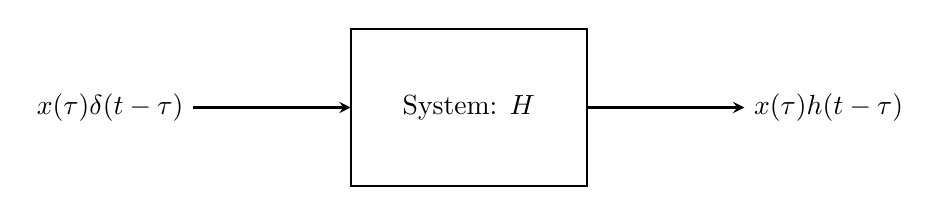
\begin{tikzpicture}[>=stealth, x=1cm, y=1
cm]
  % Draw the system box
  \draw[thick] (0,0) rectangle (3,2);
  \node at (1.5,1) {System: $H$};

  % Input arrow and label
  \draw[->, thick] (-2,1) -- (0,1);
  \node[anchor=east] at (-2,1) {$x(\tau)\delta(t - \tau)$};

  % Output arrow and label
  \draw[->, thick] (3,1) -- (5,1);
  \node[anchor=west] at (5,1) {$x(\tau)h(t - \tau)$};
\end{tikzpicture}
\caption{Impulse response of a system: output $h(t)$ when input is $\delta(t)$. What is the output for a general input $x(t)$?}
\label{fig:convolution-buildup}
\end{figure}
So, using the integral representation of the input signal, we can write the output of the system as
\[
y(t) = \int_{-\infty}^{\infty} x(\tau) h(t - \tau) d\tau.
\]
This integral is called the convolution integral, and it is denoted by the symbol $*$. Therefore, we can write the output of the system as
\[
y(t) = x(t) * h(t).
\]
\begin{popquiz}
    Write the discrete-time version of the convolution integral.
    \popqsplit
    In discrete-time, the convolution integral becomes a sum. Therefore, we can write the output of the system as
    \[
    y[n] = \sum_{k=-\infty}^{\infty} x[k] h[n - k].
    \]
    This sum is called the convolution sum, and it is also denoted by the symbol $*$.
\end{popquiz}